\documentclass[abstracton,12pt]{scrreprt}

\usepackage[
backend=bibtex,
style=alphabetic,
]{biblatex}


\usepackage{etoolbox}
\usepackage{array, booktabs}
\usepackage{graphicx}
\usepackage[x11names,table]{xcolor}
\usepackage{caption}
\newcommand{\foo}{\color{LightSteelBlue3}\makebox[0pt]{\textbullet}\hskip-0.5pt\vrule width 1pt\hspace{\labelsep}}
\makeatletter
\patchcmd{\scr@startchapter}{\if@openright\cleardoublepage\else\clearpage\fi}{}{}{}

\usepackage{graphicx}
\usepackage{wrapfig}
\usepackage{amsmath}
\usepackage{chronology}
\addbibresource{bib.bib}
%opening
\titlehead{Department of Informatics, University of Zürich}
\subject{\vspace*{2cm}MSc Thesis Proposal}
\title{Project Description: Enumerating and Maintaining groups of queries in FIVM}
\author{
	Johann Schwabe\\[-5pt]
	\scriptsize Matrikelnummer: 17-726-724\\[-5pt]
	\scriptsize Email: \texttt{johann.schwabe@uzh.ch}
}
\date{\vspace*{2cm}July 26, 2020}

\publishers{
	\small supervised by Prof.\ Dr.\ D.\ Olteanu and Dr. H.\ Zhang \\[5cm]
	\begin{tikzpicture}[overlay]
		\node at (-3,-3) {
\includegraphics[height=1.5cm]{IFIlogo}};
		\node at (4.5,-3) {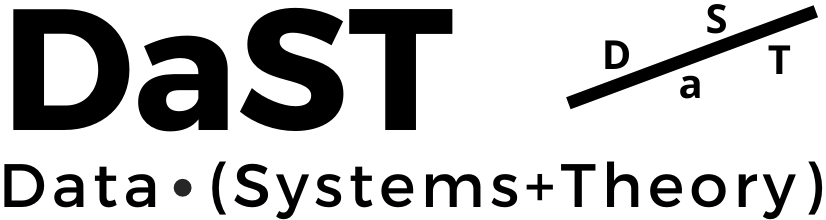
\includegraphics[height=1.5cm]{dast-logo}};
	\end{tikzpicture}
}

\begin{document}
\maketitle



\chapter{Problem and Motivation}
Most datasets in modern real-world applications are constantly changing. Tuples are inserted or removed to reflect changes in the real world. Thus, views on these datasets used to display relevant information concisely to people or applications need to be updated on data changes. For many applications, it is crucial to have up-to-date views all the time. While traditional database engines are optimised to compute joins of relations as fast as possible, they underperform when tuples are inserted or removed from the relations as they recompute the joins. 

Contrary, F-IVM is a database engine focused on efficiently computing joins of relations and maintaining the results under updates. F-IVM is limited to maintaining and enumerating a single query, which is often not enough. For groups of queries, an independent instance of F-IVM would need to run for every individual query. To enhance the performance of F-IVM, computations between queries can be shared. This allows for efficient execution of non-q-hierarchical queries that could individually not be efficiently computed. This finding calls for theoretical backing on which groups of queries can profit from the shared computation. The contributions of this thesis will be twofold. First, a characterisation of those groups of queries that admit together constant update time and constant enumeration delay will be presented. Second, an extension of the F-IVM system with support for such groups of queries along with benchmarking against prior work will be implemented.

 F-IVM achieves efficient enumeration and maintenance of individual queries by generating partial results of the join in the form of views. These views together form a view tree that can be enumerated to list the join result. While many view trees exist for a query, the resulting performance can vary greatly. Additionally, it uses Rings to factorize the computation and avoid costly intermediate joins when possible. In incremental view maintenance, a tradeoff needs to be made between enumeration time and update time. Eagerly updating means that more computations are done on every update to the dataset, leading to faster enumeration. Contrary, lazy updation does little computation on update but requires longer enumeration time per tuple. The best approach depends on the expected number of updates and enumerations and is thus application specific. 
 
 For some join queries, a variable order, used to define the structure of the view tree, can be found so that these queries can be maintained in O(1) and enumerated in O(1), which is the best efficiency possible. Maintaining a query in O(1) means that upon adding or removing any tuple to any relation, constant time is needed to update the internal data structure of the database system. Equivalently, enumeration time in O(1)  defines that at any time, the next tuple in the result can be generated in constant time. Queries with constant enumeration and maintenance time are exactly those that are hierarchical and free-dominant. They are called q-hierarchical \autocite{CQAP}.  Using rings for the aggregation operations improves computations times and allows for many different in-database computations with the same database engine. \autocite{FIVM} gives examples for rings to compute Matrix Chain Multiplication, Gradient Computation and Factorized result representation.
\autocite{FIVM}

\chapter{Approach and Contribution}
F-IVM currently generates individual executables for each query. However, parts of the computation could be shared for multiple queries on the same dataset. In examples, it was even shown that a q-hierarchical query and a non-q-hierarchical query could be, if computed sequentially, enumerated and maintained in O(1) per resulting tuple/update. If the queries were computed independently, this efficiency would not be possible. We call the groups of queries that benefit from shared computation and achieve asymptotic enumeration and maintenance speed of O(1) Cascading Q-Hierarchical. Sharing computation not only allows the efficient execution of cascading non-q-hierarchical queries but can also accelerate the already efficient q-hierarchical queries or enhance the performance of non cascading q-hierarchical queries.  An example of cascading q-hierarchical queries is Equation \ref{Queries}. While $Q_1$ is hierarchical and (trivially), free-dominant, $Q_2$ is neither and thus not q-hierarchical.

\begin{equation}
\begin{split}\label{Queries}
	&Q_1(x,y,z) = R_1(x,y), R_2(y,z)	\\
	&Q_2(x,z,w) = R_1(x,y), R_2(y,z), R_3(z,w)
\end{split}
\end{equation}
\begin{figure}
	\centering
	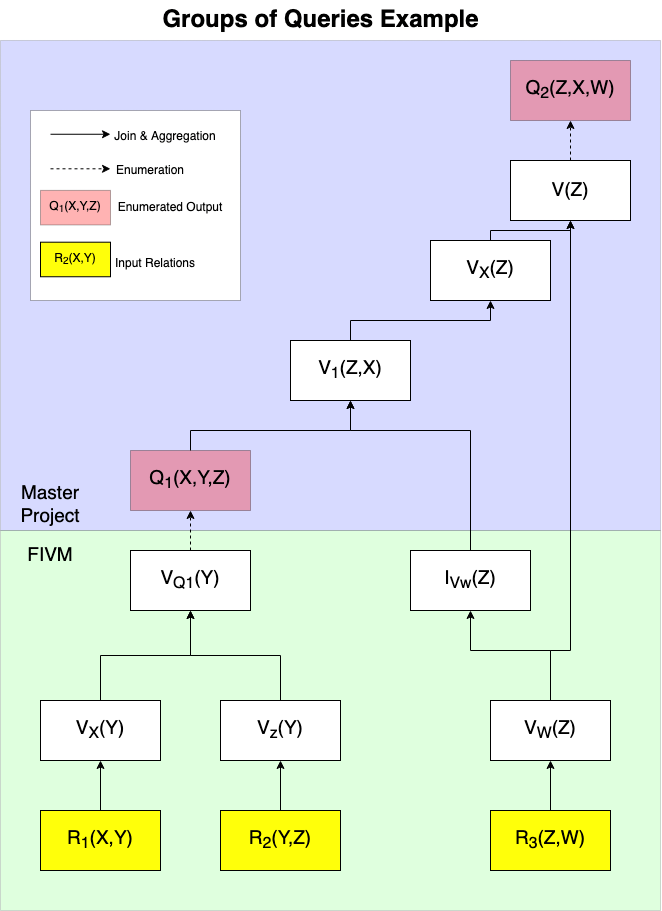
\includegraphics[width=0.5\textwidth]{GroupsOfQueriesDiag}
	\caption{Possible view tree for the group of queries in Equation \ref{Queries}}
	\label{fig:ViewTree}
\end{figure}

Assuming a view $V_1(x,z)$ were given, $Q_2$ could be simplified to $Q_2(x,z,w) = V_1(x,z),$ $ R_3(z,w)$, which is again q-hierarchical. In this example, $V_1(x,z)$ can be easily generated while enumerating $Q_1$ by projecting away $y$. Thus both Queries can be enumerated efficiently. A possible view tree for the combined computation of these queries is given in Figure \ref{fig:ViewTree}: From $R_1$, x is aggregated away, and from $R_2$, z is aggregated away, resulting in $V_X(y)$ and $V_Z(y)$. These two are then joined into $V_{Q1}(y)$.  $V_{Q1}(y)$ is the root of the view tree for $Q_1$.  From $R_3(z,w)$, $w$ is aggregated away to get $V_W(z)$. Using an indicator projection ,$I_{Vw}(Z)$ can be assembled.  By looking up the $X$ and $Z$ corresponding to a $Y$ in  $V_{Q1}(y)$, the result of $Q_1$ can be enumerated. During this enumeration, for every output tuple, whether the $z$ is within $I_{Vw}(Z)$ is checked. If it is, the tuple $(z,x)$ is added to the new view $(V_1(z,x))$. From this view, $x$ is aggregated away ($V_X(Z)$), and it is joined with $V_W(z)$ to create $V(z)$. By looking up $z$ in $V_1(z,x)$ and $R_3(z,w)$, the result of $Q_2$ can be enumerated.


The above example illustrates the possibility of sharing computation between queries to compute non q-hierarchical queries efficiently. It is to be determined for which groups of queries this is possible. Finding a theorem determining the compatibility of queries will be the first essential contribution of the thesis. F-IVM currently only supports the generation of the views marked green in Figure \ref{fig:ViewTree}. The remaining parts, marked in blue, will be implemented on top of F-IVM and represent another contribution of this thesis. The implementation will be tested and benchmarked on several groups of queries over real-world datasets.


\chapter{Timeline}

\begin{table}[h]
\renewcommand\arraystretch{1.4}\arrayrulecolor{LightSteelBlue3}
\captionsetup{singlelinecheck=false, labelfont=sc, labelsep=quad}
\caption{Timeline}\vskip -0.7ex
\begin{tabular}{@{\,}r <{\hskip 2pt} !{\foo} >{\raggedright\arraybackslash}p{5cm}}
	\toprule
	\addlinespace[1ex]
	25.1.23 & Start of thesis\\
	01.2.23 & Start theoretical part\\
	01.4.23 & Start implementation\\
	01.6.23 & Benchmarking\\
	14.6.23 & Final writing \\
	25.7.23 & End of thesis\\
\end{tabular}
\end{table}
\newpage
\printbibliography
\end{document}
